\documentclass[conference]{IEEEtran}
%\usepackage{graphicx}
\usepackage[dvipdfmx]{graphicx}
%\usepackage{latexsym}
\usepackage{slashbox}
%\usepackage{multirow}
\usepackage{url}
\usepackage{color}
\usepackage{colortbl}
\usepackage{hhline}
\usepackage{flushend}
\usepackage{verbatim}
%\usepackage{hyperref}
\usepackage{enumerate}
\usepackage[sort&compress]{natbib}
\usepackage{subfigure}
\usepackage{framed}
%\usepackage{natbib}

\newcommand{\todo}[1]{{\color{green}{\textbf{TODO: [#1]}}}}
\newcommand{\yasu}[1]{{\color{red}{\textbf{Yasu says: [#1]}}}}
\newcommand{\emad}[1]{{\color{blue}{\textbf{[#1]}}}}
\newcommand{\Emad}[1]{{\color{blue}{\textbf{[#1]}}}}
\newcommand{\revised}[1]{{\color{red}{#1}}}
\newcommand{\para}[1]{{\color{magenta}{\textbf{This paragraph:}}} [#1]}

%\newcommand{\revised}[2]{\marginpar{\fbox{#2}}{\color{red}{#1}}}

\newcommand{\nbf}[1]{
%  \noindent{\textit{\textbf{#1}}}
  \noindent{\textbf{#1}}
}

\newcommand{\conclusionbox}[1]{%
	\vspace{2mm}
  \noindent
	\framebox[0.48\textwidth][c]{%
		\parbox[b]{0.45\textwidth}{%
			{\em #1}
		}
	}
}

% Set bibliography title
%\renewcommand\refname{REFERENCES}
%\renewcommand\bibsection{\section{\refname}}

\newcommand{\ea}{{\em et al.}}
\newcommand{\smallsection}[1]{\vspace{1mm}\noindent {\bf #1}.\hspace{2mm}}
\newcommand{\emphsection}[1]{\vspace{1mm}\noindent \underline{{\em #1}.}\hspace{2mm}}


% Reduce bibliography font size
%\def\bibfont{\normalsize} %normalsize should be default
% small or footnotesize

% Reduce space between references
%\setlength{\bibsep}{3.2pt} %3.5pt should be default


\begin{document}

\title{Going Beyond Code and Bugs:\\Trends and Future Directions }

\author{\IEEEauthorblockN{Yasutaka Kamei}
\IEEEauthorblockA{Principles of Software Languages Group (POSL)\\
Kyushu University, Fukuoka, Japan\\
Email: kamei@ait.kyushu-u.ac.jp}
\and
\IEEEauthorblockN{Emad Shihab}
\IEEEauthorblockA{Department of Computer Science and Software Engineering\\
Concordia University, Montr\'eal, Canada\\
Email: eshihab@encs.concordia.ca}}

% make the title area
\maketitle

% As a general rule, do not put math, special symbols or citations
% in the abstract
\begin{abstract}
As software systems play an increasingly important role in our lives, their complexity continues to increase; making software quality assurance efforts very difficult. Therefore, a significant amount of recent research focused on the prioritization of software quality assurance efforts. One line of work that has been receiving an increasing amount of attention for over 40 years is software defect prediction, where predictions are made to determine where future defects might appear. Since then, there are many studies and many accomplishments in software defect prediction. At the same time, there remain many challenges that face software defect prediction. To blaze future trails in software defect prediction, the paper aims to accomplish three things. First, we provide a brief overview of software defect prediction and its various components. Second, we revisit the challenges of software prediction models as they were seen in the year 2000, in order to reflect on our accomplishments since then. We also highlight our accomplishments and recent trends, as well as, discuss the game changers that had a significant impact on software defect prediction. Third, we highlight some key challenges that lie ahead in the near (and not so near) future in order for us as a research community to tackle these future challenges.

%\todo{Next version.} We love pragmatic solutions that practitioners can use to maximize their software quality with the least amount of resources.
%--- ``deriving practical guidelines for developing more reliable software systems''


\end{abstract}

\IEEEpeerreviewmaketitle

% Here is Yasu't note
\begin{comment}
I did not start my research career in year 2000!
 2001-2005: Bachelor 
 2005-2007: Master
 2007-2009: PhD

As a first draft, we drop a literature review part due to time-consuming work.
\end{comment}

%%%%%%%%%%%%%%%%%%%%%%%%%%%%%%%%%%%%%%%%%%%%%%%%%%%%%%%%%%%
%What is technical debt and self-admitted technical debt
Technical debt is term first coined by Cunningham in 1993 to refer to the phenomena of taking a shortcut to achieve short term development gain at the the cost of increased maintenance effort in the future \cite{Cunningham1992WPM}. The technical debt community, organized through the managing technical debt workshop \cite{Falessi2014MTD}, has studied many aspects of technical debt, including its detection \cite{Zazworka2013CSE}, impact \cite{Zazworka2011MTD}
and the appearance of technical debt in the form of code smells \cite{Fontana2012MTD}. Most recently, we developed an approach to identify technical debt from code comments, referred to as self-admitted technical debt (SATD). SATD refers to the situation where developers know that the current implementation is not optimal and write comments alerting the inadequacy of the solution.

% What people did and what is the impact of TD. What they found.
In the last few years, an increasing amount of work has focused on SATD. In particular, our prior work focused on the detection of SATD~\cite{Potdar2014ICSME} and the classification of different types of SATD and the development of datasets to enable future studies on SATD~\cite{Maldonado2015MTD}. Other work by Bavota and Russo performed an empirical study of SATD on a large number of Apache projects showed that SATD is prevalent in open source projects, is long lived and is increasing over time. A study by Wehaibi et al. \todo{cite Wehaibi} examined the impact of SATD on quality and found that SATD does not necessarily relate to more defects, however, it does make the software system more complex. 

%However, very little work focused on interest. Also, why is calculating interest difficult
Based on these prior findings, we measure and quantify the effect of SATD. In particular, we measure the amount of \emph{interest} caused by SATD. Although the metaphor of technical debt has been well studied, to the best of our knowledge, the quanitification of interest of technical debt has not been examined before. Measuring the interest if technical debt is non-trivial since it requires, in addition to the detection of the technical debt, the tracking of the debt over time and the development of a measure to accurately quantify this debt.

% What we do  and how we calculate interest
In this paper, we first propose the use of code metrics, in particular \todo{add}, as a measure of interest. We 
 
% Main contributions
The main contributions of the paper are three-fold.

\begin{itemize}
\end{itemize}

% Organization of the paper
\smallsection{Paper Organization} To purse the goal of this paper, the paper is organized as follows. 
Section \ref{background} explains the overview of defect prediction models.
Section \ref{past} revisits what challenges were in Year 2000.
%Section \ref{trends} assesses what state the research trend is in.
%Section \ref{game_changers} presents game changers, which dramatically changed perspective and direction of the studies in the field of defect prediction.
Section \ref{trends} assesses what state the research trend is in and presents some of game changers, which dramatically changed perspective and direction of the studies in the field of defect prediction.
Section \ref{challenges} highlights some key challenges for future.
Section \ref{conclusion} draws conclusions.


%%%%%%%%%%%%%%%%%%%%%%%%%%%%%%%%%%%%%%%%%%%%%%%%%%%%%%%%%%%
\section{Background} \label{background}
%\emph{Prevention is better than cure.}
\para{Technical debt}

\cite{Guo2011ICSM}: they track technical debt items and access its impact (cost) among incurred, deferred and paid. That said, they focused on only one event (WebDav protocol is not supported) and 

\para{Software Evolution: We calculate interest by looking at the difference size of two versions. In other words, this work is one of lines of software evolution.}

%%%%%%%%%%%%%%%%%%%%%%%%%%%%%%%%%%%%%%%%%%%%%%%%%%%%%%%%%%%
\section{Past: Year 2000} \label{past}
%\emph{Today is yesterday's pupil.}
%\para{We summarize what the weakness and need for extension of the traditional defect prediction approaches in 2000 (millennium).} We introduce them by following our scheme (i.e., data collection, metrics calculation, model building and model evaluation).

In order to grasp the level of accomplishments, it is necessary to look back and examine the challenges that faced the software defect prediction in the past. In particular, we look back since the year 2000, when Fenton \ea~\cite{Fenton1999TSE} published the seminal survey on software defect prediction. To enhance readability, we organize this section along the four dimensions used in Section~\ref{background}, i.e., data, metrics, modelling and performance evaluation.

%We summarize 10 needs for extension of the traditional defect prediction approaches in 2000 (millennium). We introduce them by following our scheme of Section~\ref{background} (i.e., data collection, metrics calculation, model building and model evaluation).

Figure \ref{fig:whole_picture} shows the overview of past, trends and future in defect prediction studies.

\begin{figure*}
  \centering
  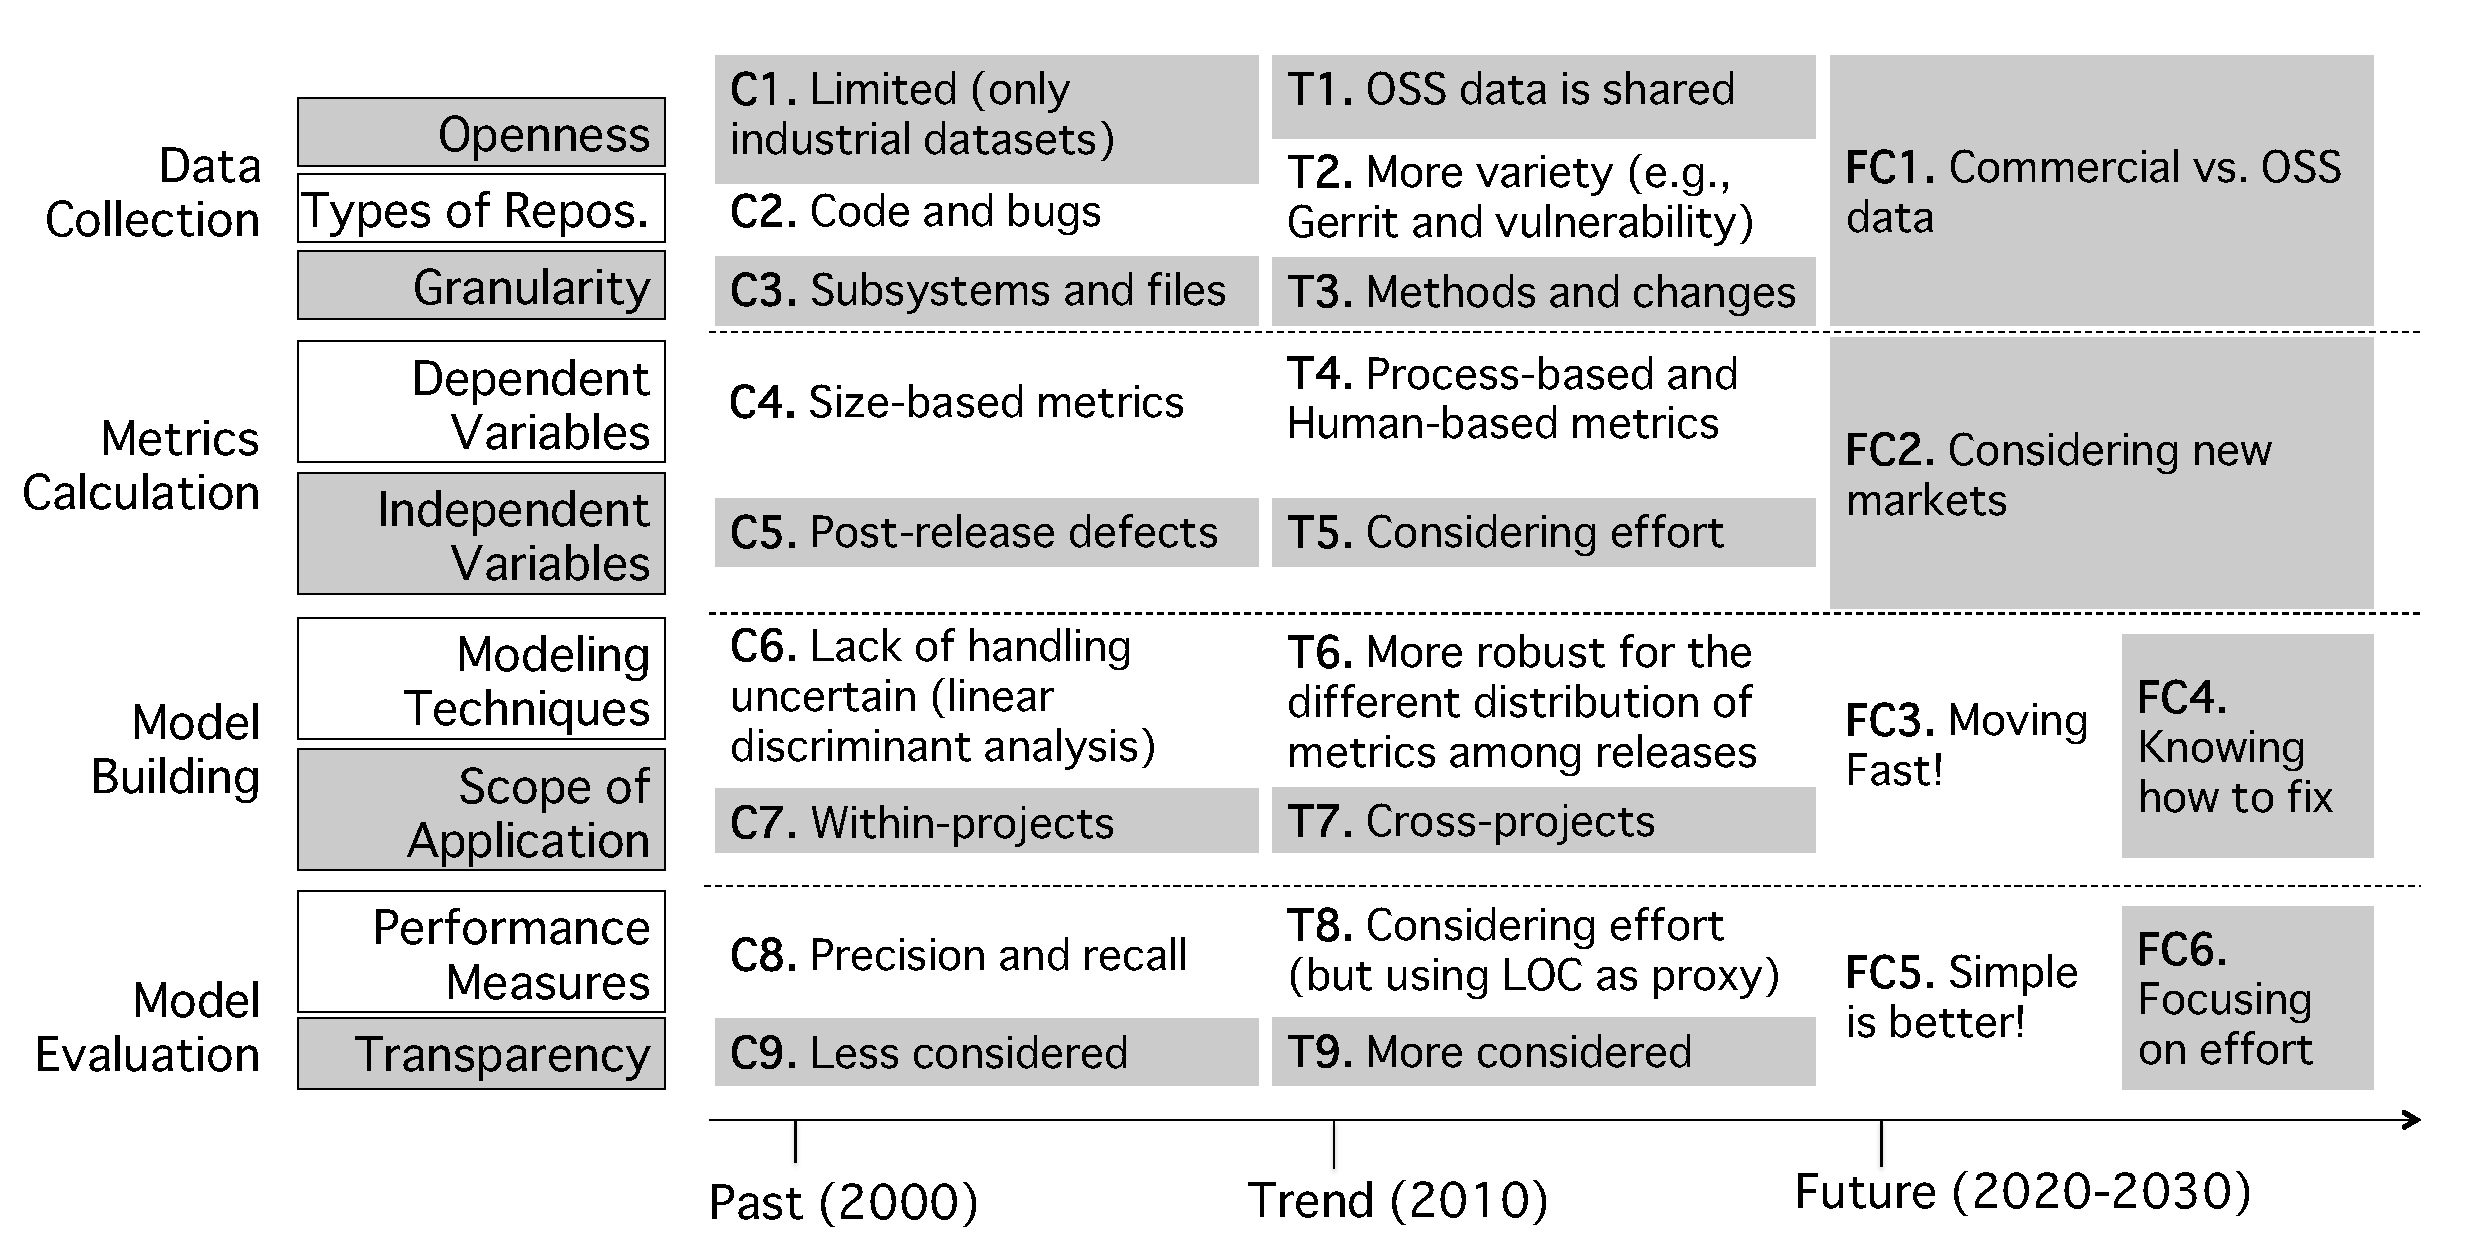
\includegraphics[width=.9\textwidth]{figures/whole_pitcture}
  \caption{Overview of Past, Trends and Future in Defect Prediction Studies \label{fig:whole_picture}}
\end{figure*}

%%%%%%%%%%%%%%%%%%%%%%%%%%%%%%%%%%%%%%%%%%%%%%%%%%%%%%%%%%%
\subsection{Data}

\smallsection{Challenge 1: Lack of Availability and Openness}
In the year 2000, one of the main challenges facing all data-driven approaches (including software defect prediction) was the lack of data availability. Software defect prediction was done only within several select, and perhaps forward-thinking, companies using their industrial data.
However, since software companies almost never want to disclose the quality of their software, researchers can never obtain the datasets used in previous studies. This was a major challenge.

Validating this challenge, a survey of software defect prediction papers published between the years 2000-2010~\cite{Shihab2012PhD} showed that 13 our of 14 defect prediction papers published between the years 2000-2002 conducted their studies using datasets collected from industrial projects. Obviously, these dataset were not shared. The other paper that used open source software data~\cite{Denaro2002ICSE}, used data from the Apache Web server project, however, they never made their datasets publicly available. This shows that back in the year 2000, data availability and openness was a real challenge facing the software defect prediction community.
% \emad{Yasu: is this what you wanted to say?}
% \yasu{Yes}

\smallsection{Challenge 2: Lack of Types of Repositories}
In addition to the lack of availability of data, the variety of the data was very limited as well. In the year 2000, most papers used data from source code and bug repositories, because those repositories provided the most basic information for building defect prediction models. For example, all 14 defect prediction studies between the years 2000 and 2002 used source code and bug repositories only~\cite{Shihab2012PhD}. Clearly, this shows that not only was data scarce, it was also very difficult to come up with different types of data.

%Nowadays, several types of repositories are available for defect prediction models, such as software review repositories (Gerrit) and vulnerability repositories. \emad{Yasu, I am not sure we should talk about what happens nowadays since we don't do that in the data collection part. What do you think?}
%\yasu{I agree}

% now we also use email, software inspection, testing.

\smallsection{Challenge 3: Lack of Variety of Granularity}
In addition to data availability and variety, the granularity of the data was another issue that faced software defect prediction work in the 2000s. The prediction unit (granularity) heavily depends on the data that is collected from the software repositories and used to build the defect prediction models. There are different levels of granularity such as the subsystem~\cite{Zimmermann2008ISSRE}, file~\cite{Dambros2010MSR} or function~\cite{Kim2007ICSE} level. 

%The finer the granularity, the better, since we will be able to narrow down the defect to a smaller code unit. Of course, the tradeoff here is that making predictions at a fine granularity is more difficult since, since for example, it is much more difficult to predict defective methods compared to subsystems, i.e., it is much easier when your unit of prediction is bigger.
%\emad{not sure if we need the last 2 sentences since the end of the next paragraph says the same thing I think}
%\yasu{I agree. I would drop the last 2 sentences.}

In 2000, the majority of studies were performed at the subsystem or file levels. Only one paper~\cite{Wong2000SPE} of the 14 defect prediction studies between 2000 and 2002 performed its prediction at the function level ~\cite{Shihab2012PhD}. The main reason for most studies performing their prediction at high levels of granularity is that repository data is often given at the file level and can be easily abstracted to the subsystem level. Although performing predictions at the subsystem and file levels may lead to better performance results~\cite{Schroter2006ISESE,Zimmermann2007}, the usefulness of the defect prediction studies becomes less significant (i.e., since more code would need to be inspected at high levels of abstraction).

%\emad{I think we should add a conclusion box here to summarize the challenges of data collection in 2000s}
%\yasu{Agree}

\conclusionbox{Software defect prediction studies in the 2000s were facing the challenges for the lack of data availability, variety and granularity.}

%%%%%%%%%%%%%%%%%%%%%%%%%%%%%%%%%%%%%%%%%%%%%%%%%%%%%%%%%%%
\subsection{Metrics}
Due to the limitations on data in the 2000s, there were several implications on the metrics and the type of metrics that were used in software defect prediction models.

\smallsection{Challenge 4: Lack of Variety of Independent Variables \textemdash Size-Based Metrics}
Size-based metrics (i.e., product metrics) are metrics that are directly related or derived from the source code (e.g., complexity or size). In the 2000s, a large body of defect prediction studies used product metrics to predict defects. The main idea behind using product metrics is that, for example, complex code is more likely to have defects. However, as Fenton and Neil mentioned~\cite{Fenton2000ICSE} in future of software engineering in 2000, while size-based metrics correlated to the number of defects, they are poor predictors of defects (i.e., there is no linearly relationship between defect density and size-based metrics). Furthermore, several studies found that code complexity metrics tend to be highly correlated with each other and with the simple measure of Lines of Code (LOC)~\cite{Fenton2000ICSE}.

%\emad{Also, we need to transition better to the post-release defects. One way would be to divide it into independent and dependent variables.}
%\yasu{I agree}

% now we use process, social, experience as metrics.

\smallsection{Challenge 5: Lack of Variety of Dependent Variables \textemdash Post-Release Defects}
Generally speaking, the majority of defect prediction studies predicted post-release defects. In fact, between 2000 and 2002, 13 of 14 defect prediction studies used post-release defects as a dependent variable~\cite{Shihab2012PhD}. Although the number of post-release defects is important and measures the quality of the released software, it is the only criteria for software quality. The fact that so many studies focused on the prediction of post-release defects is a limitation of software defect prediction work.

%\emad{same as above, we should also add a conclusion of the limitations for metrics in the 2000s.}
%\yasu{Agree}

\conclusionbox{In the 2000s, software defect prediction was focusing on size-based metrics as independent variables and post-release defects as dependent variable.}

%\smallsection{Many metrics?}

% we have some techniques to solve this problem
% http://yogi.se.rit.edu/~emad/pubs/Shihab_ESEM2010.pdf
% but is there any paper that use such 40 metrics at same time?

%%%%%%%%%%%%%%%%%%%%%%%%%%%%%%%%%%%%%%%%%%%%%%%%%%%%%%%%%%%
\subsection{Model building}
\smallsection{Challenge 6: Treating Uncertainty in Model Inputs or Outputs}
In the 2000s, linear regression and logistic regression models were often used as modeling techniques because they are simple modeling techniques. Defect prediction models assume that the distributions of the metrics in the training and testing datasets are similar~\cite{Turhan2009ESE}. However, in practice, the distribution of metrics can vary among releases. 
If the distribution vary among releases, linear regression and logistic regression models
specialize only in training data and fail prediction into testing data.

%\emad{I am not sure what you want to say here. What I would say is most use linear and logistic reg since they are simple. However, they are limited and more sophisticated techniques needed to be explored since 1) they could perform better (e.g., random forests)and 2) they may help us better understand our solutions (e.g., decision trees)}
%\yasu{What you would say is same as what I wanted to say.}

% we now have ensemble learning techniques.

\smallsection{Challenge 7: Building Models for Projects in the Initial Development Phases}
In the 2000s, most software defect prediction studies trained their models on data from the same project, usually from early releases. Then, the trained models were used to predict defects in future releases. In practice however, training data may not be available for projects in the initial development phases or for legacy systems that have not archived historical data. How to deal with projects that did not have prior project data was an open challenge in the 2000s.

%To overcome the limited availability of training data, recent work has introduced cross-project defect prediction models, i.e., models trained using historical data from other projects~\cite{Turhan2009ESE}. However, in 2000, defect prediction studies focused on only within-projects (i.e., models trained using historical data from same projects).
% \emad{I would remove this paragraph since it is not talking about the challenges man.}
% \yasu{Agree}

% we now also work on cross-projects.

%\smallsection{They are essentially black box models that hide crucial assumptions from potential users}
% decision tree or some models.

\conclusionbox{The challenges of model building in the 2000s were how to deal with projects that 
did not have the similar distributions of the metrics between training and testing datasets 
and did not have prior project data.}

%%%%%%%%%%%%%%%%%%%%%%%%%%%%%%%%%%%%%%%%%%%%%%%%%%%%%%%%%%%
\subsection{Model evaluation}

\smallsection{Challenge 8: Lack of Practical Performance Measures}
Once the prediction models are built, one of the key questions is how well do they perform. In the 2000s, many defect prediction studies empirically evaluated their performance using standard statistical measures such as precision, recall and model fit (measured in $R^2$ or deviance explained). Such standard statistical measures are fundamental criteria to know how well defect prediction models predict and explain defects. However, in some cases other more practical criteria needed to be considered. For example, how much effort is needed to address a predicted defect or the impact of a defect may need to be taken into consideration.

%  Recently, several studies try to evaluate their models using practical performance measurement.

\smallsection{Challenge 9: Lack of Transparency/Repeatability}
In the 2000s, due to the lack of availability and openness of the datasets, other studies were not able to repeat the findings of prior studies. Such lack of repeatability misses the critiques of current and new research~\cite{Shepperd2013TSE} and \cite{Ghotra2015ICSE}. Hence, comparing the performance of a technique with prior techniques was nearly impossible in the 2000s.

% Some paper shares their data and scripts to re-run their analysis.

\conclusionbox{In the 2000s, defect prediction studies were lacking the practical performance measures in industrial perspective and transparency in academic perspective.}

%%%%%%%%%%%%%%%%%%%%%%%%%%%%%%%%%%%%%%%%%%%%%%%%%%%%%%%%%%%
\section{Trends} \label{trends}

The challenges faced in the 2000s were the focus of the research that followed. Solutions to many of the challenges mentioned in Section~\ref{past} were proposed and major advancements were accomplished. In this section, we highlight some of the \emph{recent} trends in the area of software defect prediction. \revised{Furthermore, we discuss the game changers that pursed the accomplishments and had a significant impact on software defect prediction.}
Similar to the previous sections, we organize the trends along the four dimensions, data, metrics, models and performance evaluation.

%%%%%%%%%%%%%%%%%%%%%%%%%%%%%%%%%%%%%%%%%%%%%%%%%%%%%%%%%%%
\subsection{Data}

\smallsection{Trend 1: Availability and Openness}
Once the software defect prediction community realizes that data availability and openness is a key factor to its success, many defect prediction studies started sharing not only their data, but even their analysis scripts. For example, in 2004, NASA MDP (metrics data program) shared 14 datasets that are measured during the software development of NASA projects through the PROMISE repository (we will discuss the PROMISE repository later in this section)~\cite{promiserepo}. The NASA datasets were some of the first public datasets from industrial software projects to be shared in the defect prediction domain. Similarly, Zimmermann \ea ~\cite{Zimmermann2007}, D'Ambros \ea ~\cite{Dambros10MSR}, Jureczko \ea ~\cite{Jureczko2010PROMISE}, Kamei \ea ~\cite{kamei2013tse} and many others shared their open source data. In fact, many conferences now have special tracks to facilitate the sharing of datasets and artifacts. For example, the ESEC/FSE conference~\cite{FSE2015} now has a replication package track that encourages authors to share their artifacts. The MSR conference now has a dedicated data showcase track that focuses on the sharing of datasets that can be useful for the rest of the community.

Reflecting back, the recent trend of data sharing and openness have in many ways helped alleviate the challenge that existed in the early 2000s. That said, not all data is being shared; our community needs to continue to nourish such efforts in order to make data availability and openness a non-existing issue. 

%share the datasets that they collect from 3 versions of the Eclipse project. In 2010, share the datasets collected from 48 releases of 15 open source projects. provide the datasets measured from more than 450 versions of 5 open source software. The datasets include not only product metrics but also process metrics. In 2013,  share their change-level datasets that are collected from 6 open source software projects.


%There are only a part of papers that open their datasets.
%We believe that defect prediction studies are solving the problem in 2000 (i.e., software defect prediction studies was the lack of availability and openness of datasets).
% \emad{I am not sure what this is trying to say.}
% \yasu{The paragraph is "Reflecting back" is what I wanted to to say}


\smallsection{Trend 2: Types of Repositories}
In addition to using the traditional repositories such as bug and code repositories, recent studies have also explored other types of repositories. For example, Meneely and Williams~\cite{Meneely2010ESEM} leveraged the vulnerabilities database to examine the effect of the ``too many cooks in the kitchen'' phenomena on software security vulnerabilities. Other studies such as the study by Lee \ea ~\cite{Lee2011FSE} leveraged Mylyn repositories, which capture developer interaction events. McIntosh \ea ~\cite{McIntosh2014MSR} leveraged Gerrit data, which facilitate a traceable code review process for git-based software projects to study of the impact of modern code review practices on software quality. Other types of repositories are also being used, especially as software development teams become more appreciative of the power of data analytics.

Reflecting back, the recent trends show strong growth in the different types of repositories being used. We believe that exploring new repositories will have a significant impact on the future of software defect prediction since it will facilitate better and more effective models and allow us to explore the impact of different types of phenomena on software quality.
%\emad{Need to edit this}.



% such as selecting and editing software source, to extract and use 56 developer interaction metrics (e.g., the effort spent on a file).
%They show that the interaction metrics can outperform or improve defect prediction performance over using code or history metrics, improving F-measure by 0.2.


%They perform their case study on three open source systems (i.e., Linux kernel, PHP and Wireshark). They find that files changed by six developers or more were at least four times more likely to have a vulnerability than files changed by less than six developers.

%Through a case study of 3 open source projects, they find that code review coverage, participation, and expertise sh

% now we also use email, software inspection, testing.

\smallsection{Trend 3: Variety of Granularity}
Due to the benefits of performing predictions at a finer granularity, recent defect prediction studies have focused on more fine-grained level, such as the method level~\cite{Kim2007ICSE,Hata2012ICSE,Giger2012EMSE} and change level~\cite{Aversano2007,Kim2008TSE,kamei2013tse}. For example, Giger \ea ~\cite{Giger2012EMSE} empirically investigate whether or not defect prediction models at the \emph{method-level} works well. Another example of work that aims to perform predictions at a finer granularity is the work on change-level prediction, which aims to predict defect introducing changes (a.k.a commits). The advantage of predicting defect introducing changes, compared to subsystems or files is that a change is much smaller, can be easily assigned and contains complete information about a single change (which is important if a fix spans multiple files for example).

%The experimental results using 21 open source projects show that their prediction models can predict 88\% of defects with precision of 84\%.  
%For example of the change level, Kim \ea ~\cite{Kim2008TSE} use metrics extracted from source code changes to predict whether a change will be buggy (i.e., introduce a defect) or clean.
%They show that they can classify changes with an accuracy of 78\% and achieve an average of 60\% recall of buggy changes.

% now we also use change-level and method-level too.

\revised{
Reflecting back, the recent trends have realized that the practical value of the predictions decrease as the abstraction level increases (i.e., since more code would need to be inspected at high levels of abstraction). The recent trends show that they focus more on performing predictions at a finer level of granularity, e.g., at the method-level and change-level. 
}

\begin{oframed}
%\begin{leftbar}
\vspace{-0.2cm}
\smallsection{Game Changer 1: OSS projects} 
Open Source Initiative, which was founded in 1998 and is an organization to dedicate to promoting open source software, describes \emph{open source software is software that can be freely used, changed, and shared (in modified or unmodified form) by anyone.}~\cite{OSI}
Nowadays, there are no end of active open source software projects online supported by a huge range of people.

An OSS project is a change changer, because it opens the development history of long-lived widely-deployed software systems.
Figure \ref{fig:oss} shows that the number of papers using OSS projects is growing over time~\cite{Shihab2012PhD}. 

Other way to access such rich data source is to cooperate with commercial organization (e.g., ABB Inc,~\cite{Li2006} and Avaya~\cite{Mockus2010FSE}).
However, commercial organization in many cases is not willing to give access to the detail of its rich data source due to confidential reasons.
While another way is to use academic projects (e.g., course projects), such projects are relatively not rich comparing with commercial projects.
In short, OSS projects provide rich, extensive, and readily available software repositories. 
\end{oframed}

%-----------------------------------------------------------------------
\begin{figure}
  \centering
  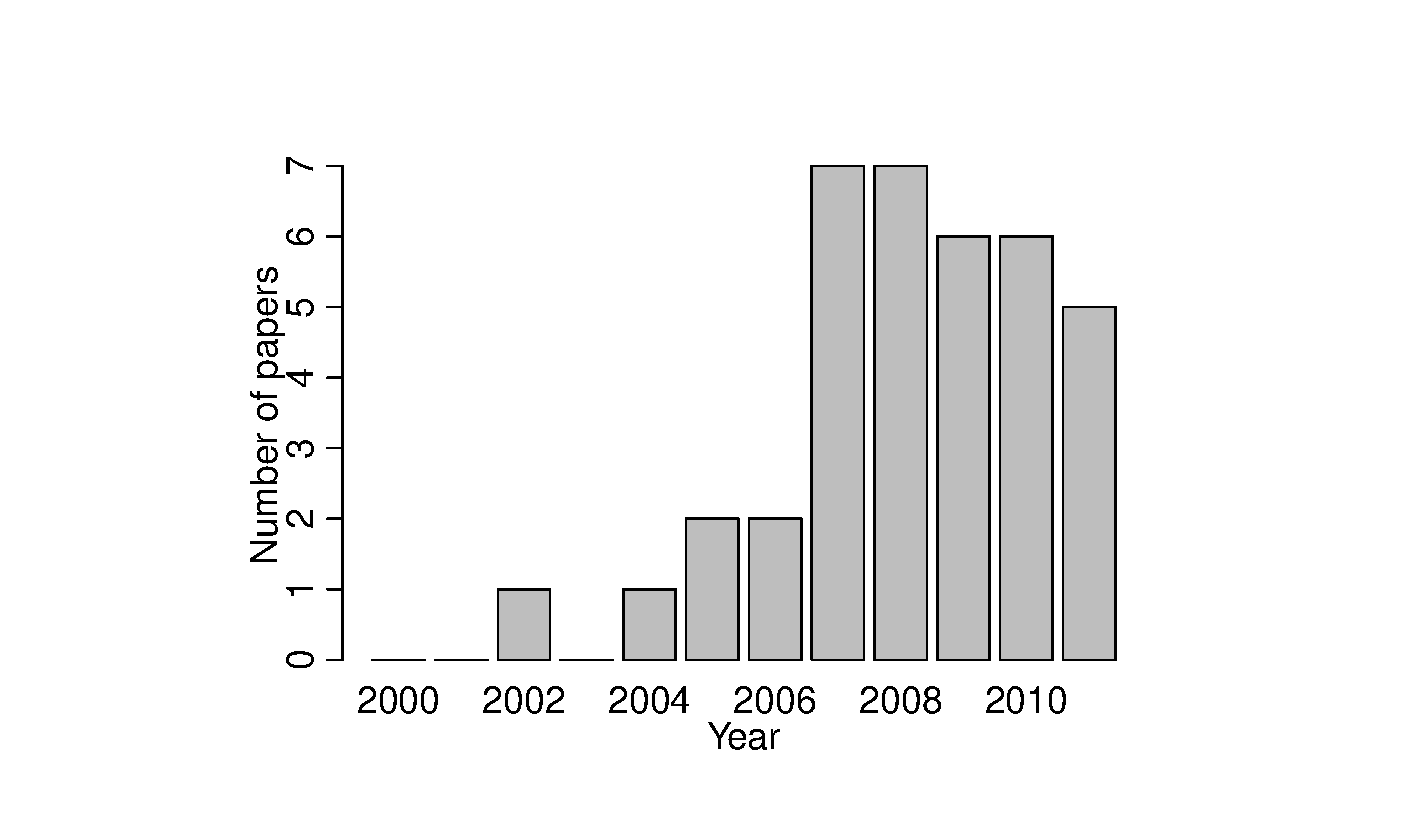
\includegraphics[trim=100 30 100 0, scale=0.5,clip]{figures/papers}
  \caption{The number of defect prediction papers using open source projects \label{fig:oss}}
\end{figure}
%-----------------------------------------------------------------------


\begin{oframed}
%\begin{leftbar}
\vspace{-0.2cm}
\smallsection{Game Changer 2: The PROMISE repository}
The PROMISE repository is a research data repository for software engineering research datasets and offers free and long-term storage for our research datasets~\cite{promiserepo}.
We can find more than 45 datasets about defect prediction in the PROMISE repository.
The PROMISE repository starts to share the samples of the Metrics Data Program, which was run by NASA for collecting static code measures in 2002, as version 1 in 2004.
The PROMISE repository is currently version 4 from 2014 and is upgraded to terabyte size.

The PROMISE repository is a game changer, because we can skip our own data collection processes and obtain promptly pre-processed and valuable datasets.
This dramatically speeds up the progress of defect prediction studies. 
The repository is in widespread use. For example, as of 2010, there are 73 papers that use the repository on IEEE Explorer~\cite{promiserepo}.
\end{oframed}

%%%%%%%%%%%%%%%%%%%%%%%%%%%%%%%%%%%%%%%%%%%%%%%%%%%%%%%%%%%
\subsection{Metrics}

\smallsection{Trend 4: Variety of Independent Variables}
In addition to using code metrics, recent software defect prediction used process metrics, which measure the change activity that occurred during the development of a new release, to build highly accurate defect prediction models~\cite{NagappanICSE05_2,Moser2008ICSE}. The idea behind using process metrics in defect prediction is that the process used to develop the code may lead to defects, hence the process metrics may be a good indicator of defects. For example, if a piece of code is changed many times or by many people, this may indicate that it is more likely to be defect prone.

Although much of the current research used process metrics to predict defects, other metrics have been proposed in the literature. For example, studies explored design/UML metrics~\cite{Briand2002TSE, Erika2010ICSE, Nugroho2010MSR} (which capture the design of the software system), social metrics~\cite{Bird2009ISSRE} (which combine dependency data from the code and from the contributions of developers), organizational metrics~\cite{Mockus2010FSE} (which capture the geographic distribution of the development organization, e.g., the number of sites that modified a software artifact) and ownership metrics~\cite{Bird2011FSE} (which measure the level of ownership of a developer to a software artifact.

%\revised{
%Reflecting back, the recent trends show the impact of not only code based metrics, but also a lot of variety of independent variables on software defects. We believe that exploring new metrics will be worth to the future of software defect prediction since defect prediction models need to capture the characteristics of the defects that our new environments raise (e.g., smart phones).
%}

Reflecting back, we saw a very clear evolution in the way software defect prediction work uses metrics. Initially, most metrics were deigned to help improve the prediction accuracy. However, more recently, studies have used defect prediction to examine the impact of certain phenomena, e.g., ownership, on code quality. Such studies have pushed the envelope in metric design and contributed significantly to the body of empirical work on software quality in general.
%\emad{I suggest we refactor what you revised to what I wrote here.}
% now we use process, social, experience as metrics.

\smallsection{Trend 5: Variety of Dependent Variables}
In the early 2000s, most studies used post-release defects as a dependent variable~\cite{Briand2002TSE,Denaro2002ICSE}. More recently however, many studies started to focus on different types of dependent variables that span much more than post-release defects. For example, Shihab \ea ~\cite{Shihab2011FSE} focused on predicting defects that break pre-existing functionality (breakage defects) and defects in files that had relatively few pre-release changes (surprise defects). Meneely and Williams~\cite{Meneely2010ESEM} built models to predict software security vulnerabilities. Garcia \ea~\cite{Garcia2014MSR} predicted blocking defects, which block other defects from being fixed. 
\revised{Furthermore, researchers have proposed to perform predictions at the change-level, focusing on predicting defect-inducing changes~\cite{Kim2008TSE, Mockus2000BTJ}. The prediction can be conducted at the time when the change is submitted for unit test (private view) or integration. Such immediate feedback ensures that the design decisions are still fresh in the minds of developers~\cite{kamei2013tse}.}

%\emad{should we discuss some of the change-level prediction stuff here?}

%and Chen \ea~\cite{Chen2014MSR} conduct an empirical study of dormant defects, which are introduced in a version of the software system, but are not found until much later.

Reflecting back, it seems that many of the recent studies have realized that not all defects are equal and that there are important defects that are not post-release defects. The recent trends show that different types of dependent variables are being considered, which take into account different stakeholders \revised{different timing}. For example, the prediction of blocking defects clearly shows that helping the developers in the main goal, which is different from the traditional defect prediction studies which mainly focused on the customer as the main stakeholder. \revised{The prediction of defect-inducing changes shows that predictions are made early on, comparing with the traditional studies which have their drawbacks (i.e., predictions are made too late in the development cycle).}

%\emad{should we discuss some of the change-level prediction stuff here?}

\begin{oframed}
%\begin{leftbar}
\vspace{-0.2cm}
\smallsection{Game Changer 3: SZZ algorithm}
\'{S}liwerski \ea ~proposed the SZZ algorithm\footnote{SZZ stands for the capital letter of authors' last name, \'{S}liwerski, Zimmermann and Zeller.}~\cite{sliwerski2005} that extracts whether or not a change introduces a defect from VCSs. The SZZ algorithm links each defect fix to the source code change introducing the original defect by combining information from the version archive (such as CVS) with the bug tracking system (such as Bugzilla).

The SZZ algorithm is a game changer, because it provides new data source for defect prediction studies. Without the SZZ algorithm, we can rarely access the information about when a change induces a defect and conduct empirical studies on defect prediction models.
When developers submit their revision for adding functionality and modifying defects to VCSs in their project, they enter their comments (e..g, fix bug \#1000) related to their revision in log messages.
However, there is no comments to detect that a change induces a defect (e.g., introducing defects), because developers 
have no intention of introducing defects and introduce them wrongly.
Therefore, before SZZ algorithm was proposed, it is difficult to automatically recover new data source (i.e., change-level bug information). 

Today (September 2015), the paper~\cite{sliwerski2005} is cited by more than 400 papers according to Google Scholar\footnote{\url{https://goo.gl/lUiGbR}}. The algorithm is not only used for making dataset, but also opens to a new research topic (e.g., improving the accuracy of the algorithm~\cite{Kim2006ASE}).
\end{oframed}
%\end{leftbar}

%%%%%%%%%%%%%%%%%%%%%%%%%%%%%%%%%%%%%%%%%%%%%%%%%%%%%%%%%%%
\subsection{Model building}
\smallsection{Trend 6: Treating Uncertainty in Model Inputs or Outputs}
%\emad{Yasu, we need to explain what the issue is here....you go directly into ensemble learning, but it is not clear why. We should start by giving some background and highlight the problem first man.}
As we mentioned in Section \ref{past}, defect prediction models assume that the distributions of the metrics in the training and testing datasets are similar~\cite{Turhan2009ESE}. However, in practice, the distribution of metrics can vary among releases. 
To treat with projects that did not have the similar distributions of the metrics between training and testing datasets, recent defect prediction studies have used ensemble techniques.
One of the frequently-used ensemble techniques is random forests classifiers that consist of a number of tree-structured classifiers~\cite{Guo2004ISSRE,mende2009,Kamei2010ICSM}. New objects are classified from an input vector that is composed of input vectors on each tree in the forest. Each tree casts a vote at the input vector by providing a classification. The forest selects the classification that has the most votes over all trees in the forest.

The main advantages of random forest classifiers are that they generally outperform simple decision trees algorithms in terms of prediction accuracy. Also, random forest classifiers are more resistant to noise in data~\cite{Marks2011PROMISE}.

Reflecting back, the recent trends of using ensemble techniques (e.g., random forests) migrates the problem that, if the distribution of metrics vary among releases, simple modeling techniques fail prediction due to specializing only in training data.

%\smallsection{Building Models for Projects in the Initial Development Phases}
\smallsection{Trend 7: Building Cross-Project Defect Prediction Models for Projects in the Initial Development Phases}
%\emad{I think we should rename this section to cross-project defect prediction since that is what it is really about.}
%\yasu{I agree}
The majority of studies in the early 2000s focused on within-project defect prediction. This means that they used data from the same project to build their prediction models. However, one major drawback with such an approach that was recently highlighted is the fact that within-project defect prediction requires sufficient historical data, for example, data from past releases. The requirement of historical data can be a challenge, especially for newer projects. Hence, more recently, defect prediction studies have worked on cross-project defect prediction models, i.e., models trained using historical data from other projects~\cite{Menzies2013TSE, Nam2013ICSE, Turhan2009ESE, Zhang2014MSR, Zimmermann2009FSE}, in order to make defect prediction models available for projects in the initial development phases, or for legacy systems that have not archived historical data. For example Briand \ea ~\cite{Briand2002TSE} train a defect prediction model using data from one system, and test it using data from another system.

At the beginning of cross-project defect prediction models, they show that the prediction performance for the cross-project context is lower than the within-project one. However, later on, recent work has shown that cross-project models can achieve performance similar to that of within-project models. For example, in their award wining work, Zhang \ea ~\cite{Zhang2014MSR} proposes a context-aware rank transformation method to preprocess predictors, address the variations in their distributions and showed that their cross-project models achieve performance that rivals within-project models.

Reflecting back, thanks to cross-project defect prediction models, the recent defect prediction models are now available for the projects in the initial development phases or for legacy systems that have not archived historical data.
At this point, the research community has come a long way with cross-project defect prediction, however, many questions still remain. For example, the lack of availability of industrial data leaves open the question of whether models built using data from open source projects would apply to industrial projects. At this stage, cross-project defect prediction remains as an open research area.
% \emad{should we discuss some of the change-level prediction stuff here?}
% \yasu{Already we discuss change-level prediction stuff. So I don't think we should discuss.}

\begin{oframed}
%\begin{leftbar}
\vspace{-0.2cm}
\smallsection{Game Changer 4: Weka and R}
The majority of defect prediction studies use WEKA or R. WEKA~\cite{WEKA} is a tool developed by the Machine Learning Group at University of Waikato. Weka is a collection of machine learning algorithms for data mining tasks that can be applied directly to a dataset. Another commonly used tool in defect prediction studies is R~\cite{R}. R is an open source language and environment for statistical analysis.

Weka and R are game changers, because both of them provide a wide variety of data pre-processing, statistical (linear and nonlinear modelling, classical statistical tests and classification) and support for graphical techniques. They also are open source software and highly extensible. Therefore, Weka and R are commonly used in defect prediction studies. In fact, 21\% and 8\% of the papers published in defect prediction studies between 2003 and 2011 used Weka and R as tools~\cite{Shihab2012PhD}. 
\end{oframed}

% we now also work on cross-projects.

%%%%%%%%%%%%%%%%%%%%%%%%%%%%%%%%%%%%%%%%%%%%%%%%%%%%%%%%%%%
\subsection{Model evaluation}

\smallsection{Trend 8: Practical Performance Measures}
In the early 2000s, most studies used traditional performance evaluation techniques such as precision and recall. More recently defect prediction studies have focused on more practical performance evaluations. To consider evaluation in more practical setting, recent work has considered the effort required to address the predicted software artifacts~\cite{Kamei2010ICSM, Mende2010CSMR, Menzies2010ESE}. 
For example, recent work by Kamei \ea ~\cite{Kamei2010ICSM} evaluates common defect prediction findings (e.g., process metrics vs. product metrics and package-level prediction vs. file-level prediction) when effort is considered. 
%Mende and Koschke~\cite{Mende2010CSMR} compare two strategies to include the effort treatment into defect prediction models.
%One strategy is applicable to any probabilistic classifier and the other applicable only for regression algorithms.
Mende and Koschke~\cite{Mende2010CSMR} compared strategies to include the effort treatment into defect prediction models.
Menzies \ea ~\cite{Menzies2010ESE} argue that recent studies have not been able to improve defect prediction results since their performance is measured as a tradeoff between the probability of false alarms and probability of detection. Therefore, they suggest changing the standard goal to consider effort, i.e., to finding the smallest set of modules that contain most of the errors.

Furthermore, recent defect prediction studies have also conducted an interview to better understand the defect prediction models and derive practical guidelines for developing high quality software. For example, Shihab \ea ~\cite{Shihab2011FSE} ask the opinions of the highly experienced quality manager in the project about their prediction results. Based on their opinions, the authors conclude that the defect prediction models should not only predict defect locations, but also detect patterns of changes that are suggestive of a particular type of defect and recommend appropriate remedies. 

%Bird \ea ~\cite{Bird2011FSE}  disucsed  with engineers at Microsoft based on their observation of the relationship between ownership measures and software defects.  Tan \ea ~\cite{Tan2015ICSE} have interaction with developers and identify some directions such as showing the prediction  precision on historical data.

Reflecting back, we see that more recent studies have focused on the practical value of software defect prediction and try to evaluate their models in realistic settings. We strongly support such research and see this trend continuing to grow since software defect prediction models are starting to be used in industry (e.g.,~\cite{Shihab2011FSE}).


\smallsection{Trend 9: Transparency/Repeatability}
As mentioned earlier, the software engineering community as a whole has realized the value of making studies as transparent as possible. For example, recent defect prediction studies have kept transparency for their studies, then generated a  a lively discussion (e.g., critique) of the results of the studies and led to new findings.
For example, Shepperd \ea \cite{Shepperd2013TSE} derive some comments on the NASA software defect datasets (e.g., the dataset contains several erroneous and implausible entries) and share cleaned NASA defect datasets. Then, Ghotra \ea ~\cite{Ghotra2015ICSE} revisit the findings of Lessmann \ea ~\cite{Lessmann2008TSE} that used original NASA datasets. In contrary to prior results~\cite{Lessmann2008TSE}, Ghotra \ea ~shows that there are statistically significant differences in the performance of defect prediction models that are trained using different classification techniques. Such valuable are made possible thanks to the fact that the NASA projects made their datasets available.  

\begin{comment}
\emad{I don't get how the paragraph fits/relates to this section} 
\yasu{I agree. I commented out the paragraph now.}
Furthermore, defect prediction studies are likely to lead to extension studies by sharing the datasets and scripts that the studies use in their experiment.  For example, Zimmermann \ea ~\cite{Zimmermann2007} collect the datasets including product metrics from 3 versions of the Eclipse project, conduct an empirical study on defect prediction models using their own datasets and share the datasets in their web site.
Then, Moser \ea ~\cite{Moser2008ICSE} perform a comparative analysis of the efficiency of process metrics and product metrics for defect prediction by extending the datasets (i.e., only collecting process metrics) Zimmermann \ea ~\cite{Zimmermann2007} shared.
\end{comment}

Reflecting back, we see a very healthy and progressive trend where software defect prediction studies are becoming more transparent. Such changes will only make our findings more practical and will encourage use to advance the science (not only the engineering) behind the area of software defect prediction since it allows us to repeat and scrutinize assumptions of prior studies.

% Some paper shares their data and scripts to re-run their analysis.

% Sounds nice.
% Number of papers whose title contains the string "mobil" (accounting for both "mobile" and "mobility") published in flagship software engineering venues (TSE, TOSEM, ICSE, ASE, ESEC/FSE).

% http://ieeexplore.ieee.org/Xplorehelp/#/searchingIeeeXplore/usingAdvancedSearch/commandSearch/fieldCodes



%%%%%%%%%%%%%%%%%%%%%%%%%%%%%%%%%%%%%%%%%%%%%%%%%%%%%%%%%%%
%\section{Game Changers} \label{game_changers}

\emad{As discussed, we should merge this with trendds. Once you do that, I will have a look at the trends section again.}
%%%%%%%%%%%%
% Perceived Quality
% Software is more than just developing code
% Software intelligence can bridge both worlds.

\revised{Section \ref{trends} reflected on our accomplishments of software defect prediction studies since the 2000s. In this section, we discuss the game changers that pursed the accomplishments and had a significant impact on software defect prediction.}

%%%%%%%%%%%%%%%%%%%%%%%%%%%%%%%%%%%%%%%%%%%%%%%%%%%%%%%%%%%
\subsection{Data}
\smallsection{OSS projects} 
Open Source Initiative, which was founded in 1998 and is an organization to dedicate to promoting open source software, describes \emph{open source software is software that can be freely used, changed, and shared (in modified or unmodified form) by anyone.}~\cite{OSI}
Nowadays, there are no end of active open source software projects online supported by a huge range of people.

An OSS project is a change changer, because it opens the development history of long-lived widely-deployed software systems.
Figure \ref{fig:oss} shows that the number of papers using OSS projects is growing over time~\cite{Shihab2012PhD}. 

Other way to access such rich data source is to cooperate with commercial organization (e.g., ABB Inc,~\cite{Li2006} and Avaya~\cite{Mockus2010FSE}).
However, commercial organization in many cases is not willing to give access to the detail of its rich data source due to confidential reasons.
While another way is to use academic projects (e.g., course projects), such projects are relatively not rich comparing with commercial projects.
In short, OSS projects provide rich, extensive, and readily available software repositories. 

%\para{Why are OSS projects a game changer? Because we can get long-lived development projects quickly.} 


%-----------------------------------------------------------------------
\begin{figure}
  \centering
  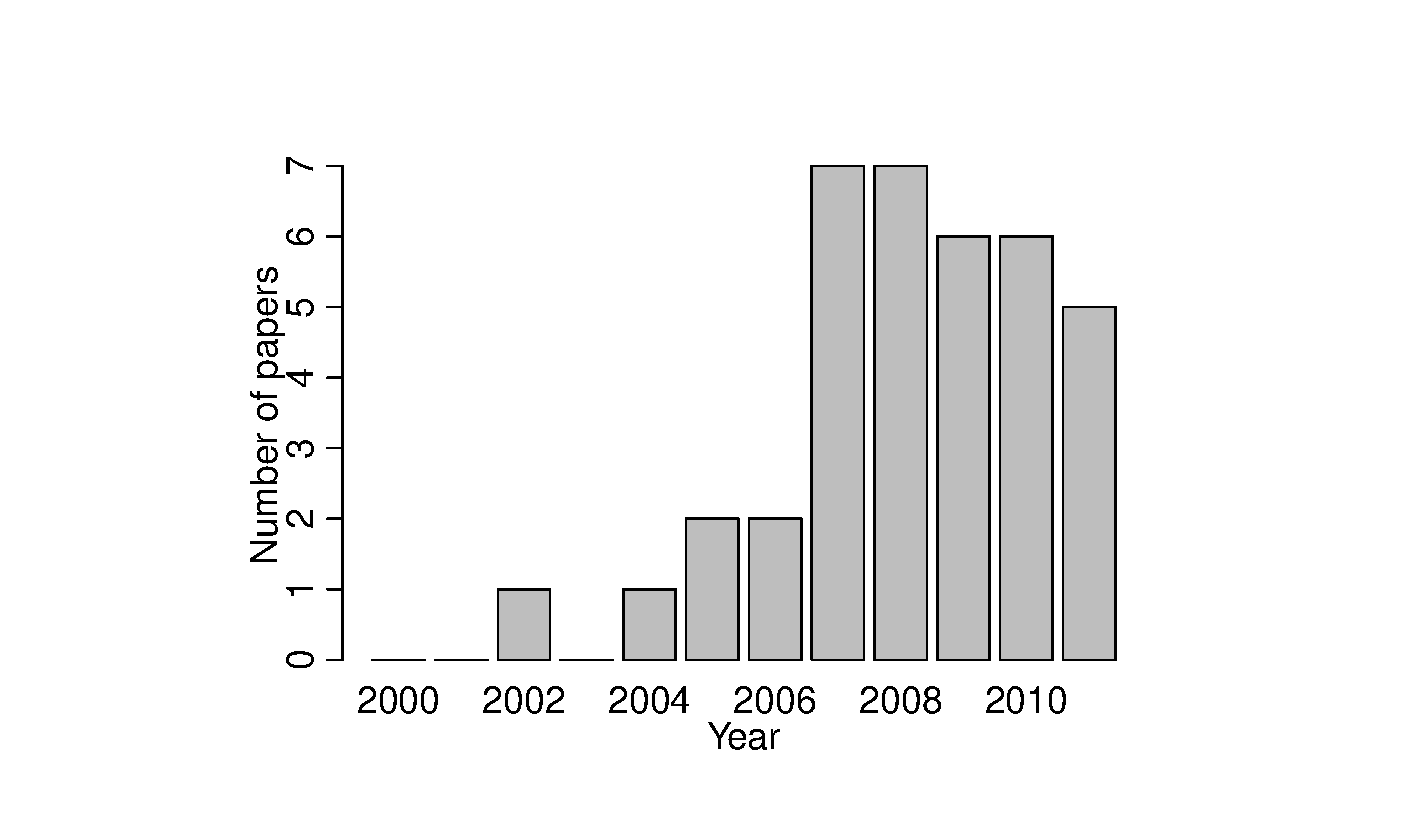
\includegraphics[trim=100 30 100 0, scale=0.5,clip]{figures/papers}
  \caption{The number of defect prediction papers using open source projects \label{fig:oss}}
\end{figure}
%-----------------------------------------------------------------------

%\para{We show some evidence that OSS projects are a game changer using the number of datasets? Emad's phd thesis.}

\smallsection{Git repositories}
Git is a well-known distributed VCS~\cite{Chacon2009Book} and is currently used in many OSS projects. Git is a game changer, because researchers copy whole repositories into their own environment very easily and quickly (just command {\tt git clone URL}), when comparing with a centralized VCS (e.g., CVS and SVN). That is, we can perform case studies using more number of projects in order to draw more general conclusions.

For example, Rahman \ea~\cite{Rahman2013ICSE} analyze the applicability and efficacy of process and code metrics from several different perspectives. They build defect prediction models across 85 releases of the git repositories of 12 large open source projects. 
Fukushima \ea~\cite{Fukushima2014MSR} empirically evaluate the performance of JIT cross-project models using data from 11 open source projects, of which 6 projects are provided
by other study ~\cite{kamei2013tse} and 5 projects (using Git repositories) needed to be collected.

\smallsection{The PROMISE repository}
The PROMISE repository is a research data repository for software engineering research datasets and offers free and long-term storage for our research datasets~\cite{promiserepo}.
We can find more than 45 datasets about defect prediction in the PROMISE repository.
The PROMISE repository starts to share the samples of the Metrics Data Program, which was run by NASA for collecting static code measures in 2002, as version 1 in 2004.
The PROMISE repository is currently version 4 from 2014 and is upgraded to terabyte size.

The PROMISE repository is a game changer, because we can skip our own data collection processes and obtain promptly pre-processed and valuable datasets.
This dramatically speeds up the progress of defect prediction studies. 
The repository is in widespread use. For example, as of 2010, there are 73 papers that use the repository on IEEE Explorer~\cite{promiserepo}.

Similar to the concept of the PROMISE repository (e.g., sharing researchers' dataset), the International Working Conference on Mining Software Repositories (MSR) has introduced a Data Showcase since 2013~\cite{MSR2013DataShowcase}. It focuses on the domain of MSR studies.

%\para{GitHub: Developer's interaction}

%%%%%%%%%%%%%%%%%%%%%%%%%%%%%%%%%%%%%%%%%%%%%%%%%%%%%%%%%%%
\subsection{Metrics}

\smallsection{SZZ algorithm}
\'{S}liwerski \ea ~proposed the SZZ algorithm\footnote{SZZ stands for the capital letter of authors' last name, \'{S}liwerski, Zimmermann and Zeller.}~\cite{sliwerski2005} that extracts whether or not a change introduces a defect from VCSs. The SZZ algorithm links each defect fix to the source code change introducing the original defect by combining information from the version archive (such as CVS) with the bug tracking system (such as Bugzilla).

Today (September 2015), the paper~\cite{sliwerski2005} is cited by more than 400 papers according to Google Scholar\footnote{\url{https://goo.gl/lUiGbR}}. The algorithm is not only used for making dataset, but also opens to a new research topic (e.g., improving the accuracy of the algorithm~\cite{Kim2006ASE}).

The SZZ algorithm is a game changer, because it provides new data source for defect prediction studies. Without the SZZ algorithm, we can rarely access the information about when a change induces a defect and conduct empirical studies on defect prediction models.
When developers submit their revision for adding functionality and modifying defects to VCSs in their project, they enter their comments (e..g, fix bug \#1000) related to their revision in log messages.
However, there is no comments to detect that a change induces a defect (e.g., introducing defects), because developers 
have no intention of introducing defects and introduce them wrongly.
Therefore, before SZZ algorithm was proposed, it is difficult to automatically recover new data source (i.e., change-level bug information). 

\subsection{Model building}

\smallsection{Weka and R}
\revised{
The majority of defect prediction studies use WEKA or R. WEKA~\cite{WEKA} is a tool developed by the Machine Learning Group at University of Waikato. Weka is a collection of machine learning algorithms for data mining tasks that can be applied directly to a dataset. Another commonly used tool in defect prediction studies is R~\cite{R}. R is an open source language and environment for statistical analysis.
}

\revised{
Weka and R are game changers, because both of them provide a wide variety of data pre-processing, statistical (linear and nonlinear modelling, classical statistical tests and classification) and support for graphical techniques. They also are open source software and highly extensible. Therefore, Weka and R are commonly used in defect prediction studies. In fact, 21\% and 8\% of the papers published in defect prediction studies between 2003 and 2011 used Weka and R as tools~\cite{Shihab2012PhD}. 
}
% 18/87 7/87

\subsection{Model evaluation}
\smallsection{Baseline?}
\todo{Baseline paper?}

%%%%%%%%%%%%%%%%%%%%%%%%%%%%%%%%%%%%%%%%%%%%%%%%%%%%%%%%%%%
%\subsection{Model building}
\begin{comment}
\smallsection{Big data analysis technique}

\smallsection{Ensemble}
\para{Year 2000, Fenton pointed out that we need to treat with uncertainty. One solution is using is ensemble techniques (e.g., Random Forest). Some paper showed that random forest outperforms others, but Lessman \ea~\cite{lessmann2008} show that there is few difference among models using statistical tests. However, recent work~\cite{Ghotra2015ICSE} replicated Lessman \ea's work using clean data sets and showed some building techniques (e.g., ensemble) outperform other models.}
\end{comment}

%%%%%%%%%%%%%%%%%%%%%%%%%%%%%%%%%%%%%%%%%%%%%%%%%%%%%%%%%%%
\section{Challenges and beyond near future} \label{challenges}

%%%%%%%%%%%%%%%%%%% sensing on the small and cheap and computing goes mainstream


As discussed, the field of software defect prediction has made many accomplishments in the recent years. However, many challenges remain and will pop up in the future do to changes in technology, data and the increasingly important role software systems continue to play.

%%%%%%%%%%%%%%%%%%%%%%%%%%%%%%%%%%%%%%%%%%%%%%%%%%%%%%%%%%%
\subsection{Data collection}
\smallsection{Future Challenge 1: Commercial vs. OSS Data}
As Section \ref{trends} shows, many researchers make use of the dataset collected from open source software projects. The main reason for using data from open source projects is that these projects archive long and practical development history and make their data publicly available. However, the generality of our findings and techniques to non open source software projects (e.g., commercial projects) is not studied in depth; in part due to the lack of availability of data. 
%The challenge is that the number of public industrial datasets is limited (e.g., only NASA datasets).

To solve this challenge, we need to make more partnership with industrial partners and have access to their repositories. The authors had some success starting projects with industry and our experience shows that starting such partnerships is easier than one might think. Especially with the hype of big data and data analysis in general, companies tend to realize that there is value in mining their data. That said, the industrial partners need to see some value with what the researchers are doing with their data, otherwise they may lose interest.

Many industrial projects have already shifted to modern software development environment (e.g., Git and Gerrit). That is, it is easy to apply our tool to their projects. Practitioners are also curious about knowing their quality using MSR techniques. 
In short, the most important thing is to have the will to start a collaboration with industrial projects. when we continue to demonstrate the value of data in software repositories and the benefits of MSR techniques for helping practitioners in their daily activities, practitioners are more likely to contact us and consider using our technique in practice. 

\begin{comment}
\smallsection{Challenge 2 (beyond near future): Reactive vs. Proactive}
When it comes to software defect prediction, many of our techniques thus far have been reactive in nature. What that means is that we observe the software development process and then use this data to predict what will happen post-release. However, in many cases practitioners would like to have predictions happen much sooner, e.g., before or as soon as they commit their changes. Doing so would make our approaches more proactive in a sense, since it will allow us to perform our predictions as the development is happening rather than waiting till it has completed.

Several studies have already started to work in this area, using metrics from the design stage \todo{cite Zeller's paper} and performing change-level defect predictions \todo{cite JIT}. However, there remains much work to do in this area. We maybe able to devise tools that not only predict risky areas or changes, but also generate tests (and possibly fixes) for these risky areas and changes. We can also devise techniques that proactively warn developers, even before they modify the code, that they are working with risky code that has had specific types of defects in the past.


Currently, we feel that we are likely to be reactive to repositories. We try to find and use the repositories that are valuable and not much studied for our studies. For example, GitHub, which is a Web-based Git repository hosting service, started in 2008, then was becoming very well-known and frequently-used Git repository hosting service around 2009-2010. Several studies~\cite{Ray2014FSE} conduct a large scale empirical studies of defect prediction by making use of the dataset collected from a pile of projects on GitHub. \emad{Yasu, I am not sure about what you wrote here man!}

We do not mention that we throw in seeking the repositories that are not much studied. The data needed to perform defect prediction is readily available as it is collected by projects for other purposes. Therefore, practitioners do not have to spend additional effort in their projects.

However, if we are proactive to repositories, we may be able to go forward into the next stage of defect prediction studies. We could propose the tool that not only archives the data needed to perform defect prediction, but also helps practitioners' daily decision-processes in modern software development organizations. Such tool (e.g., Mylyn~\cite{Lee2011FSE}) does not force them to spend additional effort in their projects. 
\end{comment}

%The feedbacks from users to software systems are valuable and fundamental for improving software quality. 

\begin{comment}
\smallsection{Developer feedbacks: Stack Overflow}
Developer feedbacks can be used for knowing how developers solve defects and 

\para{StackOverflow}
\yasu{Do you know any papers that use the data collected from StackOverflow?}
\url{here is a link: http://meta.stackexchange.com/questions/134495/academic-papers-using-stack-exchange-data/134496#134496}
\end{comment}

%%%%%%%%%%%%%%%%%%%%%%%%%%%%%%%%%%%%%%%%%%%%%%%%%%%%%%%%%%%
\subsection{Metrics calculation}

\smallsection{Future Challenge 2: Considering New Market}
The majority of software defect prediction studies used code and/or process metrics to perform their predictions. To date, this has served the community well and has helped us advance the state-of-the-art in software defect prediction.
However, comparing with year 2000, our environment has changed dramatically. Therefore, we need to tackle the defects that new environments raise. 

One example of a new market that we should tackle is mobile application fields. We use personal smart phone every day during moving and update applications from online stores (e.g., Google Play and App Store). Mobile applications play a significant role in our daily life and these applications have different characteristics compared to conventional applications that we studied in the past. These mobile application stores allow us to gain valuable user data that, till today, has not been leveraged in the area of software defect prediction. Few studies have leveraged this data to improve testing \cite{Khalid2014FSE,Khalid2015IEEESoft}. Moreover this data can be leveraged to help us understand what impacts users and in which way the user is impacted. Such knowledge can help us build better and more accurate models. We anticipate the use of user data in software defect prediction models to be an area of significant growth in the future.

Energy consumption has been one of the greatest challenge for software industries in the coming decade. Software systems are currently hosted on more than 35 million servers across thousands of data centers. Hindel published papers~\cite{Hindle2012ICSE,Hindle2012MSR} related to energy consumption (green mining) in SE conferences in 2012, then the green mining are now one of the hottest topics in SE domain~\cite{Pinto2014MSR,Sahin2014ICSME}. For future, we should develop some metrics and modeling techniques for energy consumption.

\begin{comment}
\yasu{Emad: I dropped the below, because it seems not to fit}
The fact is, research moves at a very fast speed, which is too fast for any one researcher or group. It is difficult for the one person/group to understand the problem of the modern techniques in other market fields. 
Collaborating with others from other domains can help us advance the field in a novel and speedy way. There are some good examples where collaborations with the researchers across domains have succeeded. For example, one paper~\cite{Nam2013ICSE} is published with SE researchers (1st and 3rd authors) and a data mining researcher (2nd author). The paper first applied TCA \emad{need to expand this}, which was proposed by the 2nd author and tried to reduce the data distribution difference between training and testing data, to defect prediction. However, they found that the performance of cross-project defect prediction with TCA is sensitive to normalization. Therefore, they proposed a novel transfer defect learning approach, TCA+, by extending TCA. We also find other examples where collaborations between SE researchers and natural language processing have been fruitful~\cite{Oda2015ASE}.
\end{comment}

\begin{comment}
\smallsection{Challenge 6: Getting more accurate models}
\emad{Yasu, this section is a little strange. I am not sure what you want to say here man! We already have pretty accurate models. I think we should say here that we need to be more accurate at detecting impactful bugs and build models that people can understand.}
One of the challenges is that we develop the models that always provide high accurate defect prediction models (i.e., high precision and recall).
Craig Federighi, who is Apple's senior vice president of software engineering, said the speech recognition capability in Siri now has a 5 percent word error rate, thanks to a 40 percent reduction on the part of Apple at Apple's 2015 Worldwide Developers Conference~\cite{}. While such high accurate recognition would keep the motivation of what people want to use Siri, low accurate one loses the motivation. It happens for defect prediction models. Low accurate models waste the time of developers, then developers lose the interest of the models and do not believe the alarm of the defect prediction models like \emph{The Boy Who Cried Wolf}. It is a big challenge to get 5 percent error rate for defect prediction models for future.
\end{comment}

\begin{comment}
\smallsection{Challenge 4: Collaborating with other domain researchers}
We often make use of techniques that are proposed in other research fields (e.g., data mining and AI) to build better defect prediction models~\cite{Breiman2001}. Many modern techniques are available via packages in R and Weka (e.g., Random Forest and Latent Dirichlet allocation). 
However, such techniques are sometimes not suitable for software engineering datasets due to uniqueness of SE data (e.g., the number of defect-inducing changes represents only a tiny percentage of all changes).

The fact is, research moves at a very fast speed, which is too fast for any one researcher or group. It is difficult for the one person/group to understand the problem of the modern techniques in other research fields and revise and apply them to defect prediction studies. We are likely to have more knowledge about dataset in the SE research field and how to use statistical/machine learning packages, but less mathematical knowledge to re-implement the modern techniques.

Collaborating with others from other domains can help us advance the field in a novel and speedy way. That said, it is challenging to collaborate , because we have less chance to meet the researchers in other research domain than the researchers in same domain and need to raise the research goal that both researchers are interested in.

There are some good examples where collaborations with the researchers across domains have succeeded. For example, one paper~\cite{Nam2013ICSE} is published with SE researchers (1st and 3rd authors) and a data mining researcher (2nd author). The paper first applied TCA \emad{need to expand this}, which was proposed by the 2nd author and tried to reduce the data distribution difference between training and testing data, to defect prediction. However, they found that the performance of cross-project defect prediction with TCA is sensitive to normalization. Therefore, they proposed a novel transfer defect learning approach, TCA+, by extending TCA. We also find other examples where collaborations between SE researchers and natural language processing have been fruitful~\cite{Oda2015ASE}.

In short, collaborating with the researchers in other research domains will not only help us use modern techniques, but also extend them to fit our research domain.
\end{comment}

%%%%%%%%%%%%%%%%%%%%%%%%%%%%%%%%%%%%%%%%%%%%%%%%%%%%%%%%%%%
\subsection{Model building}

\smallsection{Future Challenge 3: Moving Fast!} 
In today's fast changing business environment, the recent trend of software development is to reduce the release cycle to days or even hours~\cite{RELENG2015}.
For example, the Firefox project changes their release process to a rapid release model (i.e., a development model with a shorter release cycle) and releases over 1,000 improvements and performance enhancements with version 5.0 in 3 months~\cite{Khomh2015EMSE}.
IMVU, which is an online social entertainment website, deploys new code fifty times a day on average ~\cite{AdamsICSE2012}.

We need to think about how we integrate our research into contentious integration.
For example, O'Hearn suggested that commenting on code changes at review time makes a huge difference in helping developers than producing the bug list from batch-mode analysis because such commenting does not ask them to make a context switch to understand and act on an analysis report~\cite{CAV2015}.

The majority of quality assurance research focused on defect prediction models that identify defect-prone modules (i.e., files or packages) at release-level like batch-mode analysis~\cite{Gyimothy2005,hassan2009,Li2006,Munson1992}. Those studies use the dataset collected from previous release to build a model and derive the bug list that includes the probability of defect prone of all modules. Such model require practitioners to remember the rationale and all the design decisions of the change to be able to evaluate if the change introduced a defect.

To solve the problem that O'Hearn pointed out, we can focus on Just-In-Time (JIT) Quality Assurance~\cite{kamei2013tse,Mockus2000BTJ,Kim2008TSE}, which performs predictions at the change level. JIT defect prediction models aim to be an earlier step of continuous quality control because it can be invoked as soon as a developer commits code to their private or to the team’s workspace.

There remains much work to do in this area. As future challenge, we still need to evaluate how to integrate JIT models into actual contentious integration process. For example, we can devise the approaches that suggest how many effort developers spend to find and fix defects based on the probability of prediction (e.g., while JIT models predict that this change includes defects with 80\% of probability, the developer should work on the change for additional 30 minutes to find the defects). 
We are also maybe able to devise tools that not only predict risky areas or changes, but also generate tests (and possibly fixes) for these risky areas and changes. We can also devise techniques that proactively warn developers, even before they modify the code, that they are working with risky code that has had specific types of defects in the past.

%\para{Peter  says ``Moving fast!'' batch-mode analysis => just-in-time mode analysis}

%-----------------------------------------------------------------------
\begin{figure}
  \centering
  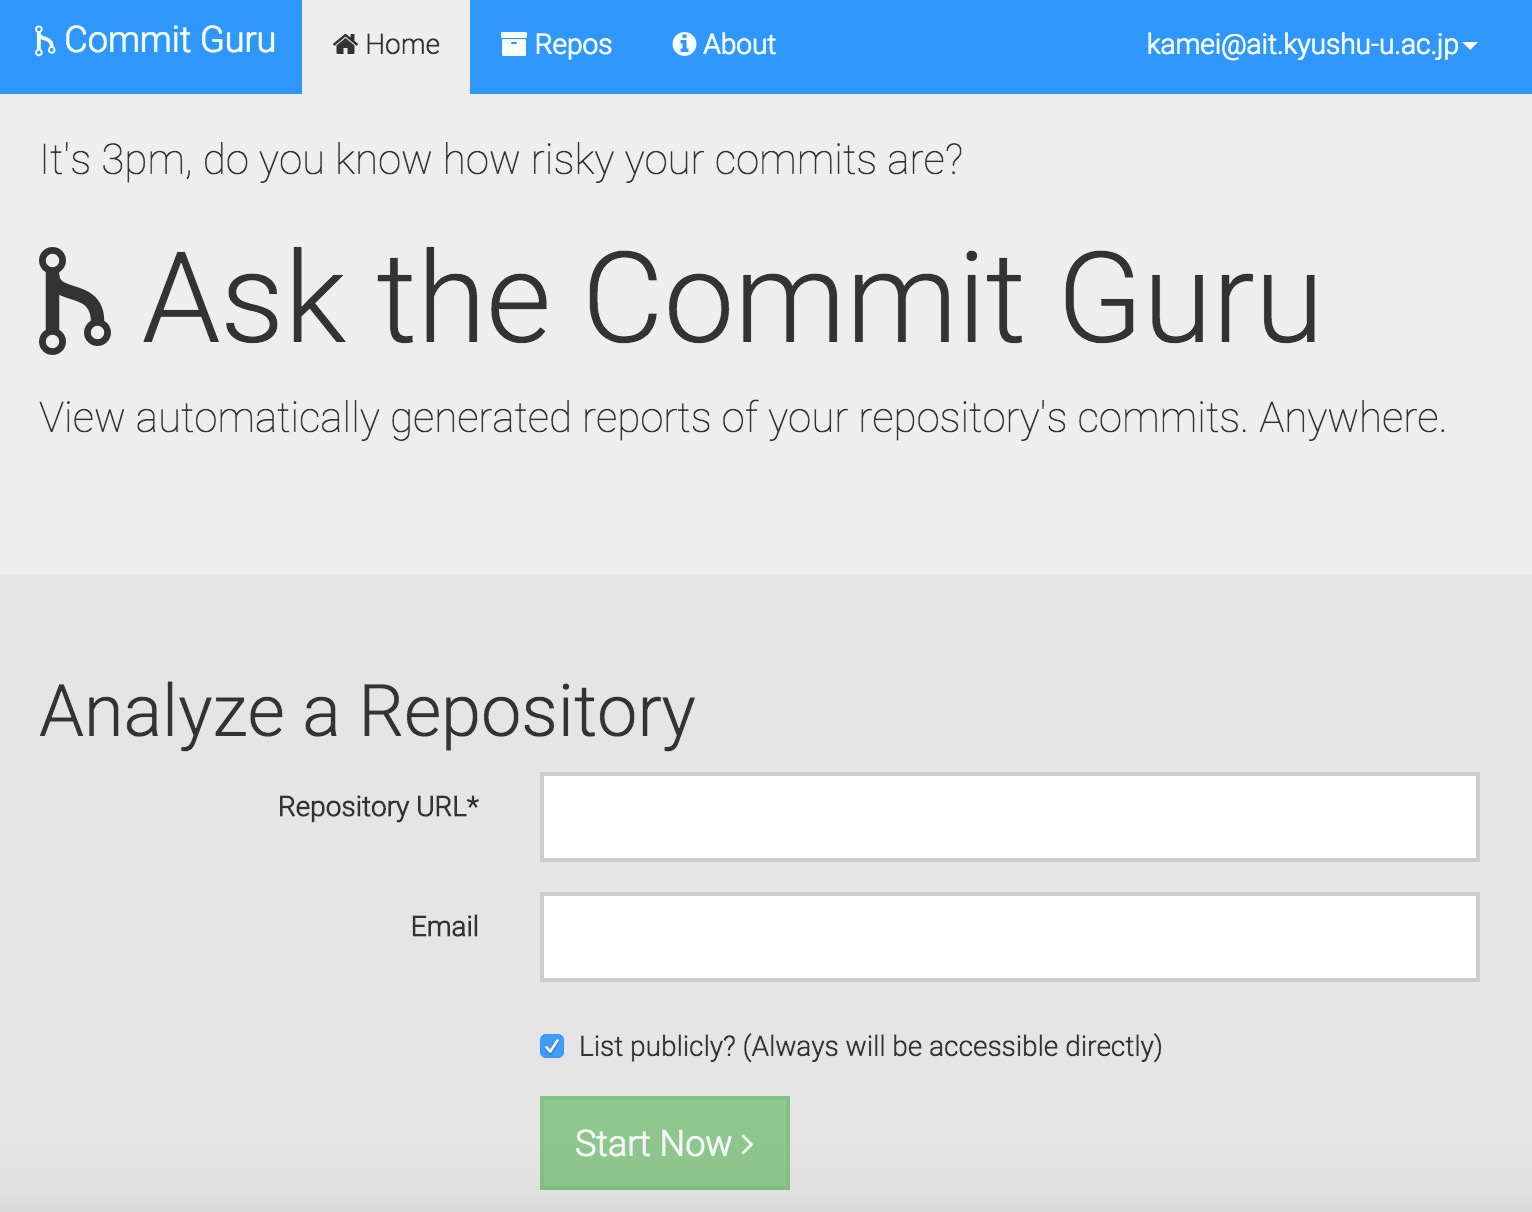
\includegraphics[width=.4\textwidth]{figures/guru1}
  \caption{Adding a Repository in Commit Guru \label{fig:guru1}}
\end{figure}
%-----------------------------------------------------------------------

%-----------------------------------------------------------------------
\begin{figure}
  \centering
  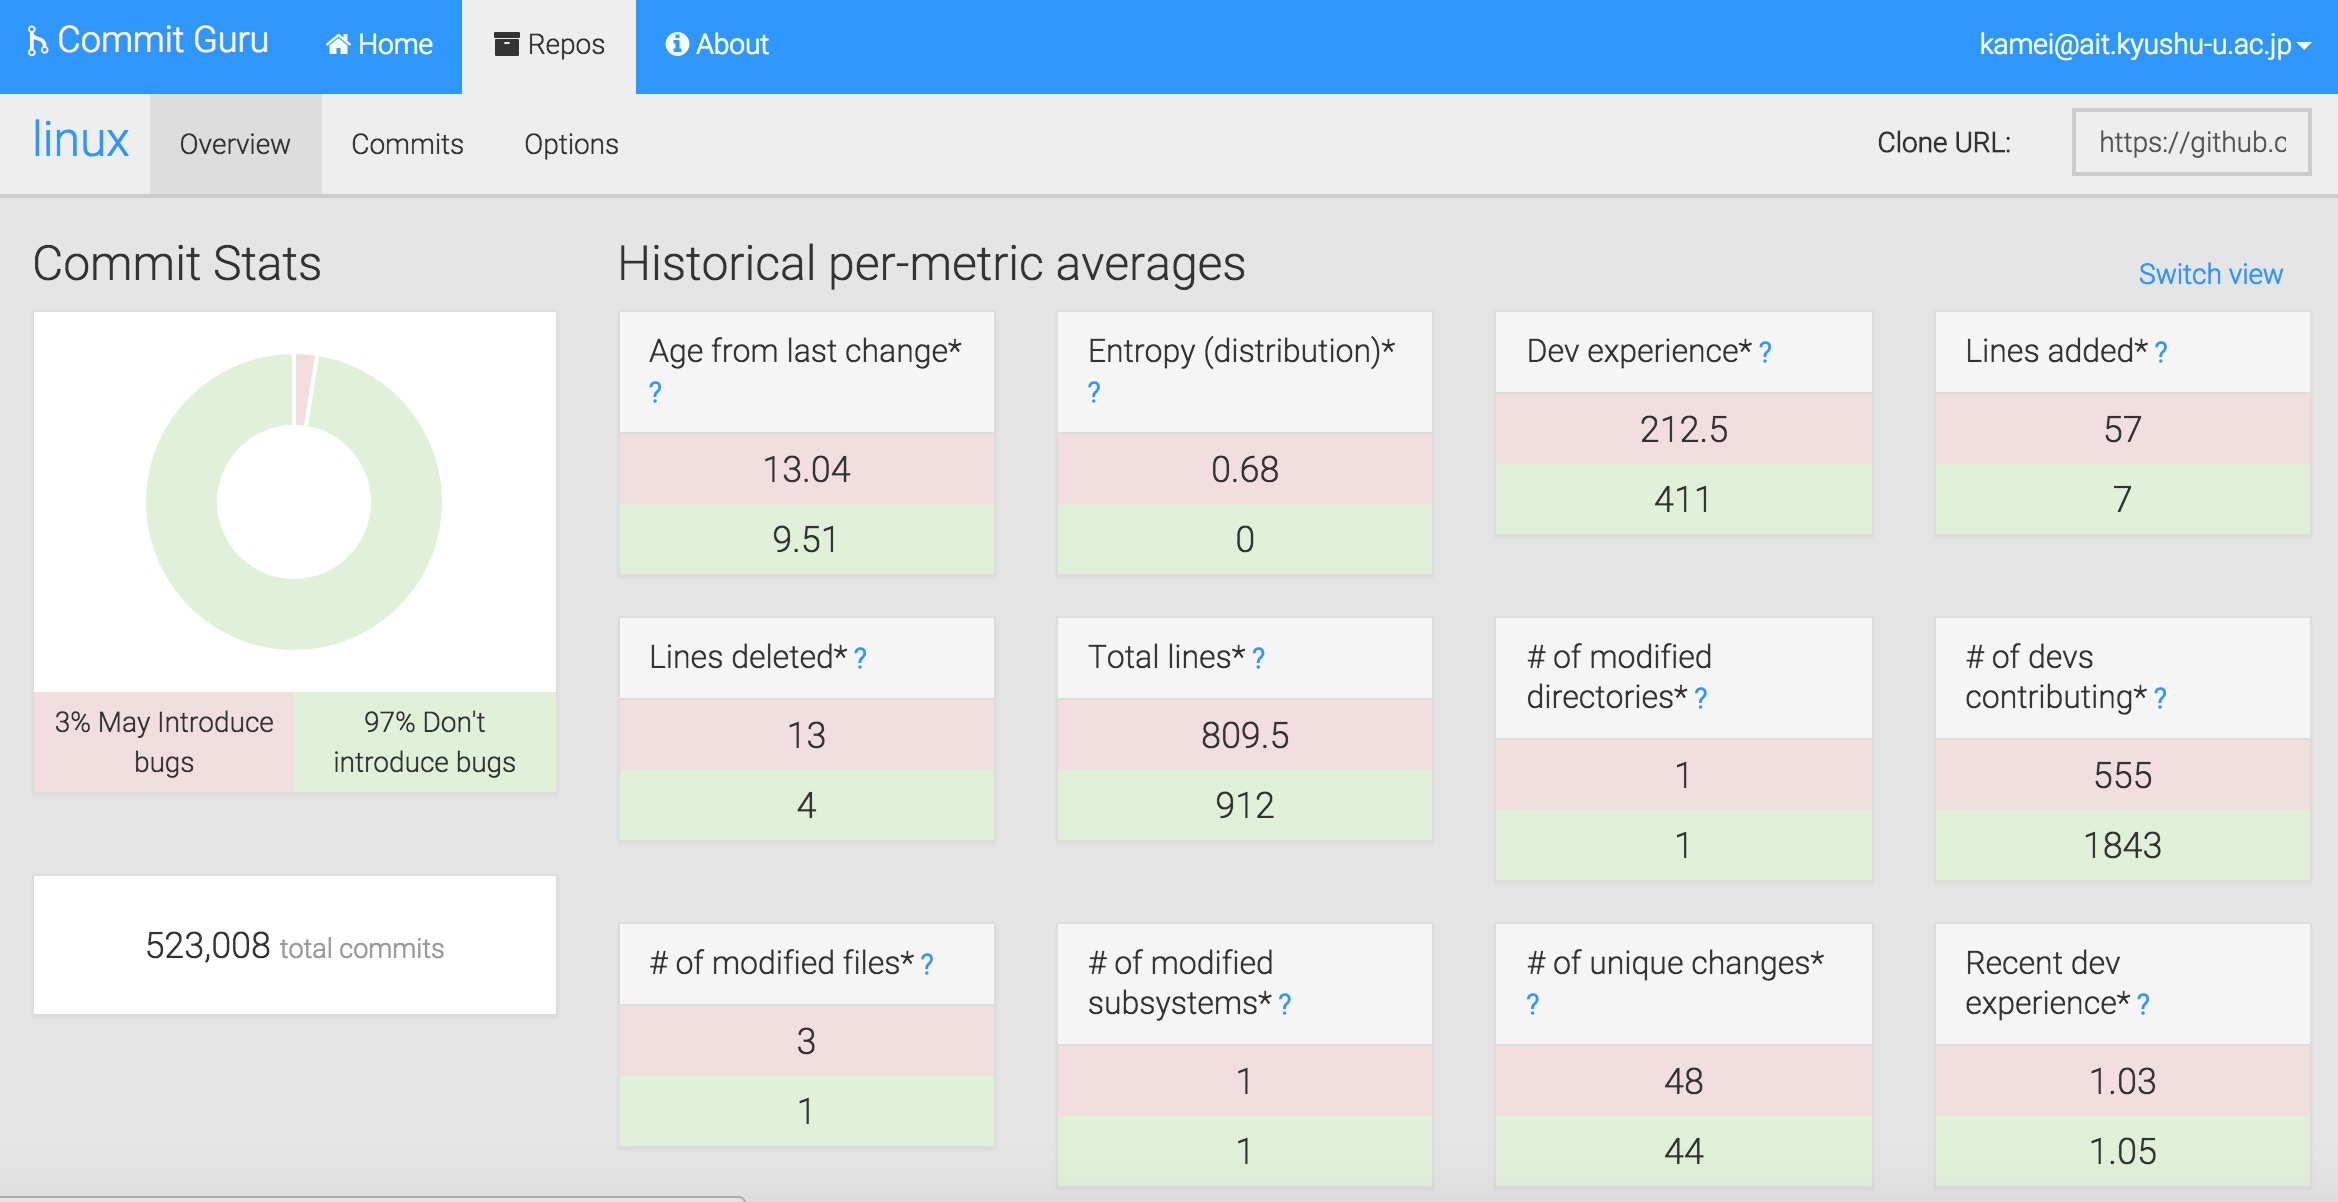
\includegraphics[width=.4\textwidth]{figures/guru2}
  \caption{Commit Statistics in Commit Guru \label{fig:guru2}}
\end{figure}
%-----------------------------------------------------------------------

\smallsection{Future Challenge 4: Knowing How to Fix a Defect!}
The main purpose of defect prediction models thus far has been three-fold: 1) to predict where defects might appear in the future and allocate SQA resources to defect-prone artifacts (e.g., subsystems and files), 2) understand the effect of factors on the likelihood of finding a defect and 3) derive practical guidelines for future software development projects. Although such models have proven to be useful in certain contexts, how to fix the defects that are flagged remains to be an open question.

Therefore, we envision that future defect prediction models will not only predict where the defects are, they will also provide information on how to best fix these defects. For future, we need to understand what kind of defects happen and why such defects happen to give developers more information to locate and fix the predicted defect. One area of research that maybe useful here is the area of automated program repair~\cite{LeGoues2012ICSE, Mechtaev2015ICSE, Nguyen2013ICSE}, which produces candidate patches for validation and deployment, when we obtain the alert of defects from defect prediction models.

%%%%%%%%%%%%%%%%%%%%%%%%%%%%%%%%%%%%%%%%%%%%%%%%%%%%%%%%%%%
\subsection{Model evaluation}

\begin{comment}
\smallsection{Challenge 9: Making our study easy to use and replicate.}

\emad{Yasu, I feel this can be combined with the point above OSS vs. commericla above.}
\Yasu{Emad, I dropped this, because this challenge is similar to trend 1.}
Recently, software engineering research papers have been trying to open their replication packages (e.g., including dataset, tool/script and ReadMe) to re-run their experiments by a third party.
The reason is mainly for (1) showing validity and transparency of the experiments and (2) giving other researchers opportunities to conduct replication studies using other datasets or compare the performance of new models with the original models using same datasets.
In ESEC/FSE 2015~\cite{FSE2015}, which is the flagship conference for Software Engineering, 16 out of 74 papers open such replication packages.\footnote{If the title of papers includes the term ``(with replication package)'', we identify that the papers open their replication packages.} 
While some defect prediction papers also open the replication packages, several papers only describe the approach (e.g., how do they measure the used metrics and how do they build prediction models) and performance (e.g., precision and recall) of the proposed models (i.e., still do not open replication packages). 

If we are interested in the models that papers propose, we want to perform replication studies to generalize the models and to know baseline performance when we propose a new model. 
Such replication studies play an important role for evolving the research field of defect prediction.
However, if we cannot access replication packages, it reduces the speed of such replication studies because we carefully read the paper and need to implement the proposed models ourselves. For future, we will try to open replication packages.
\end{comment}

\smallsection{Future Challenge 5: Simple is Better!}
%This challenge is similar to the previous challenge. While the previous challenge is more related to research interests, this challenge is more related to practical interests. We also need to consider how we simple our proposed models and replication packages are to use. When we just want to use a replication package, some types of replication packages are not suitable: (e.g., we need to carefully read README, set up some environment or modify some scripts to use them due to different environment with the replication packages). In that case, we may give up on using these techniques due to time unless we really would love to use them. We lose many chances that our proposed models are used in practice.

Recently, software engineering research papers have been trying to open their replication packages (e.g., including dataset, tool/script and ReadMe) to re-run their experiments by a third party.
The reason is mainly for (1) showing validity and transparency of the experiments and (2) giving other researchers opportunities to conduct replication studies using other datasets or compare the performance of new models with the original models using same datasets. However, for practice, we need to consider how we simple our proposed models and replication packages are to use. When we just want to use a replication package, some types of replication packages are not suitable: (e.g., we need to carefully read README, set up some environment or modify some scripts to use them due to different environment with the replication packages). In that case, we may give up on using these techniques due to time unless we really would love to use them. We lose many chances that our proposed models are used in practice.

To avoid losing the chances that our proposed models are used in practice, for future of defect prediction models, we should provide simple interface to be used such as web-base interface or virtual image \emad{Should we give simple interfaces or simple models?} \yasu{We should give simple interfaces. Commit guru is very easy to start to use.}.
Furthermore, it would be great by providing the access to our tool via REST-APIs and original scripts for the people who want to integrate the tool into their project. 
For example, Commit Guru~\cite{Rosen2015FSE} provides a language agnostic analytics and prediction tool that identifies and predicts risky software commits (Figure \ref{fig:guru1} and Figure \ref{fig:guru2}).
It is publicity available via web browsers and easy to use. The tools simply requires a URL of a Git repository that you want to analyze (Figure \ref{fig:guru1}).
Its source code is freely available under the MIT license.\footnote{It can be downloaded at \url{https://github.com/
CommitAnalyzingService/CAS_Web} (front-end) and \url{https://github.com/
CommitAnalyzingService/CAS_CodeRepoAnalyzer} (back-end).}
In short, we need to make our tools simple and extendable.

%While we need to spend a lot of effort to make our techniques available through tools that are easy to use, building such tools is likely to be less appreciated than publishing papers \emad{this may be a controversial statement}. We suggest that in the future, the number of the usage/downloads of tools should be considered in the promotion of researchers in the field of defect prediction. 
% \yasu{I agree. I dropped.}

\smallsection{Future Challenge 6: Focusing on Effort}
From the year 2000~\cite{Fenton2000ICSE}, we have one argument that we need to evaluate our prediction models in a practical setting (e.g., how much effort do defect prediction models reduce?) instead of only precision and recall. Recent studies try to tackle such problems when considering effort~\cite{Kamei2010ICSM,Mende2010CSMR}. Such studies use LOC or churn as a proxy for effort.
However, our previous studies~\cite{Shihab2013IST} show that using a combination of LOC, code and complexity metrics provides a better prediction of effort than using LOC alone. For future, we need to tackle what is the best way to measure effort in effort-aware defect prediction models. 
%\emad{dude this is about effort, but the title is perceived quality!!!}

%For user's satisfaction, online marketplaces provide many user's feedback as rating.
%We can make use of the user's feedback for our future study.


%%%%%%%%%%%%%%%%%%%%%%%%%%%%%%%%%%%%%%%%%%%%%%%%%%%%%%%%%%%
\section{Conclusion} \label{conclusion}
%\section{Conclusion} \label{conclusion}
%\section{Conclusion} \label{conclusion}
%\input{conclusion.tex}
\para{Summary of this work.}

\smallsection{Future direction}

\begin{itemize}
\item \todo{Discuss how to calculate interest.}
\item  There are several type of technical debt such as defect technical debt and design technical debt.
The previous study~\cite{Maldonado2015MTD} shows that the percentage of technical debt varies depending on the type of technical debt and the studied systems. For example, the projects that have limited time to develop features are likely to leave comments of features that need to be implemented in the future. 
To better understand the interest, we would like to analyze the interest per type of technical debt.
\item  The interest varies among technical debt. If we can understand the reason why some of technical debt has large interest, we can make use of such insights for future development. Therefore, we would like to manually investigate why some of technical debt has large interest.
\item Generally speaking, software systems are always evolving over time for implementing new functionality and fixing defects~\cite{xxx}.
Therefore, even if the size of technical debt increases, it is not clear about how the nature of software evaluation affects the interest of technical debt.
We would like to compare the impact of software evolution on methods in two groups of SATD v.s. non-SATD.
\item To operationalize our findings, we also built a tool that is able to identify and assign an interest rate to all SATD instances in a project. Our tool is publicly available and can be used by practitioners to prioritize the most impacting (i.e., highest interest) SATD.
\end{itemize}

\para{Summary of this work.}

\smallsection{Future direction}

\begin{itemize}
\item \todo{Discuss how to calculate interest.}
\item  There are several type of technical debt such as defect technical debt and design technical debt.
The previous study~\cite{Maldonado2015MTD} shows that the percentage of technical debt varies depending on the type of technical debt and the studied systems. For example, the projects that have limited time to develop features are likely to leave comments of features that need to be implemented in the future. 
To better understand the interest, we would like to analyze the interest per type of technical debt.
\item  The interest varies among technical debt. If we can understand the reason why some of technical debt has large interest, we can make use of such insights for future development. Therefore, we would like to manually investigate why some of technical debt has large interest.
\item Generally speaking, software systems are always evolving over time for implementing new functionality and fixing defects~\cite{xxx}.
Therefore, even if the size of technical debt increases, it is not clear about how the nature of software evaluation affects the interest of technical debt.
We would like to compare the impact of software evolution on methods in two groups of SATD v.s. non-SATD.
\item To operationalize our findings, we also built a tool that is able to identify and assign an interest rate to all SATD instances in a project. Our tool is publicly available and can be used by practitioners to prioritize the most impacting (i.e., highest interest) SATD.
\end{itemize}

\para{Summary of this work.}

\smallsection{Future direction}

\begin{itemize}
\item \todo{Discuss how to calculate interest.}
\item  There are several type of technical debt such as defect technical debt and design technical debt.
The previous study~\cite{Maldonado2015MTD} shows that the percentage of technical debt varies depending on the type of technical debt and the studied systems. For example, the projects that have limited time to develop features are likely to leave comments of features that need to be implemented in the future. 
To better understand the interest, we would like to analyze the interest per type of technical debt.
\item  The interest varies among technical debt. If we can understand the reason why some of technical debt has large interest, we can make use of such insights for future development. Therefore, we would like to manually investigate why some of technical debt has large interest.
\item Generally speaking, software systems are always evolving over time for implementing new functionality and fixing defects~\cite{xxx}.
Therefore, even if the size of technical debt increases, it is not clear about how the nature of software evaluation affects the interest of technical debt.
We would like to compare the impact of software evolution on methods in two groups of SATD v.s. non-SATD.
\item To operationalize our findings, we also built a tool that is able to identify and assign an interest rate to all SATD instances in a project. Our tool is publicly available and can be used by practitioners to prioritize the most impacting (i.e., highest interest) SATD.
\end{itemize}



\section*{Acknowledgment}
This research was partially supported by JSPS KAKENHI Grant Numbers 15H05306 and 25540026.

\bibliographystyle{abbrv}
%\bibliographystyle{IEEEtranN}
\bibliography{reference}


\end{document}

